\documentclass{article}

\usepackage[preprint]{neurips_2026}
\usepackage[utf8]{inputenc}
\usepackage[T1]{fontenc}
\usepackage{hyperref}
\usepackage{url}
\usepackage{booktabs}
\usepackage{amsmath,amssymb}
\usepackage{graphicx}
\usepackage{enumitem}
\usepackage{xcolor}
\usepackage{float}

\title{Head-Level Spatial Reasoning Analysis and Targeted Attention Reallocation\\
for Vision-Language Models}
\author{Your Name \\ Your Course / Program}
\date{}

\begin{document}
\maketitle

\begin{abstract}
We present a mechanism-driven study of spatial reasoning in vision-language models and use the findings to design a stronger attention intervention strategy. First, we analyze layer-17 head behavior with YOLO-grounded overlap and overlap-to-correctness AUROC on \texttt{Controlled\_Images\_A}, and find a strong negative relation between ``spatially concentrated'' heads and ``functionally useful'' heads. This suggests that final correctness is often supported by heads with weaker current spatial focus but higher latent functional potential. Second, we test a naive in-box boosting idea and show that directly forcing attention into detector regions is unstable, motivating a smoother design. We then introduce margin-guided continuous attention reallocation, which controls intervention strength by decoding confidence margin and redistributes image attention without hard clipping. Finally, we evaluate on four benchmarks (\texttt{COCO\_QA\_one\_obj}, \texttt{COCO\_QA\_two\_obj}, \texttt{VG\_QA\_one\_obj}, \texttt{VG\_QA\_two\_obj}) and observe consistent gains on harder two-object settings while preserving one-object performance. Code: \url{https://github.com/yinhhhh/spatial_reasoning_head}.
\end{abstract}

\section{Introduction}
Vision-language models (VLMs) have achieved strong performance across multimodal tasks \citep{liu2023llava,bai2023qwenvl}, yet spatial reasoning remains fragile, especially when fine-grained object relations must be inferred from visual evidence. A common line of work addresses this issue by adjusting image-side attention during decoding, with the goal of improving visual grounding and reducing relation errors \citep{adaptvis}. While such attention reweighting methods are increasingly used, most studies treat attention heads as a homogeneous resource and focus on aggregate intervention strength.

We argue that this head-agnostic view misses an important mechanistic question: \emph{do different heads contribute unequally to spatial reasoning?} If so, intervention should not only decide \emph{how much} visual attention to allocate, but also \emph{where in head space} this allocation should be concentrated. This perspective motivates our central objective: to characterize head-level functional differences in spatial reasoning and leverage them to improve downstream spatial performance.

Our core research question is:
\begin{quote}
Can we identify and reallocate spatial reasoning responsibility across heads in a way that improves spatial grounding while preserving semantic correctness?
\end{quote}
To answer this question, the paper follows a three-stage narrative:
\begin{enumerate}[leftmargin=1.2em]
  \item \textbf{Head analysis:} establish that head-level spatial roles are real and measurable, and identify which heads are already spatially effective.
  \item \textbf{Improved allocation method:} design a better strategy for distributing image attention, moving beyond naive or purely global reweighting.
  \item \textbf{Mechanism-backed validation:} use the intervention outcomes to show that heads with latent but underutilized spatial-attention potential are key targets for improving spatial reasoning.
\end{enumerate}

\section{Preliminaries}
\textbf{Attention.}
Transformer attention maps an input token sequence to contextualized representations through query, key, and value projections \citep{vaswani2017attention}. Given token features $X\in\mathbb{R}^{n\times d}$, each head computes
\begin{equation}
Q = XW_Q,\quad K = XW_K,\quad V = XW_V,
\end{equation}
and attention weights
\begin{equation}
A = \mathrm{softmax}\!\left(\frac{QK^\top}{\sqrt{d_k}}\right),
\end{equation}
followed by head output
\begin{equation}
Z = AV.
\end{equation}
Multi-head attention concatenates head outputs and applies a final linear projection.

In autoregressive decoding, the model produces next-token logits $z_t$ at step $t$, and token probabilities are obtained by
\begin{equation}
p(y_t=i\mid y_{<t},x)=\frac{\exp(z_{t,i})}{\sum_j \exp(z_{t,j})}.
\end{equation}
The generated token is selected from this distribution (e.g., greedy or sampling decoding).

\textbf{Vision-Language Models (VLMs).}
Models such as LLaVA and Qwen-VL \citep{liu2023llava,bai2023qwenvl} process an image by first encoding it with a vision backbone (typically ViT-style), which divides the image into patches and converts them into a sequence of visual features (visual tokens). These visual tokens are then projected into the language model hidden space through a connector/projection module. Finally, the visual tokens are concatenated with text tokens (prompt tokens) and fed into the decoder, so self-attention can jointly model image-text interactions in one token sequence. Our later method sections build on this standard multimodal tokenization-and-fusion pipeline.

\section{Head-Level Spatial Analysis}
\noindent Before intervention design, we first identify which heads are spatially active and which heads are functionally tied to correctness.

\textbf{Experiment settings.}
We conduct the head-level analysis on \texttt{Controlled\_Images\_A}, a synthetic and tightly controlled benchmark used in AdaptVis-style evaluation. The images are human-constructed to isolate spatial relations (e.g., left/right/on/under) with limited visual confounders, which makes it suitable for diagnosing whether attention heads truly capture spatial cues. The question set follows the AdaptVis protocol \citep{adaptvis}: GPT-4-generated relation questions in a fixed-choice format, such as ``Where is the object in relation to the anchor object?'' with options \{left, right, on, under\}. In the AdaptVis analysis, layer 17 attention is reported as most correlated with generation behavior; therefore, we focus our head-level analysis on layer 17 and use the single-box filtering protocol for reliable region attribution.

\subsection{Head-wise attention distribution (YOLO overlap)}
We first examine where each head places attention mass by computing YOLO-grounded overlap, with the following concrete procedure. For each sample, we run YOLO \citep{redmon2016yolo} to obtain the object box and retain single-box cases to reduce ambiguity. The box is expanded by a fixed scale (1.2$\times$ in our current setting) and rasterized into a binary mask $M\in\{0,1\}^{H\times W}$. For each head $h$, we extract its attention map, project/resize it to the same grid, and normalize it into a heatmap $H_h$ such that $\sum_{i,j} H_h(i,j)=1$. We then compute
\begin{equation}
\mathrm{Overlap}_h=\frac{\sum_{i,j} H_h(i,j)\,M(i,j)}{\sum_{i,j} H_h(i,j)}.
\end{equation}
Intuitively, this is the fraction of a head's attention mass that falls inside the detector-supported object region. Figure~\ref{fig:head32} visualizes a 32-head comparison for a representative sofa/armchair sample, showing strong cross-head heterogeneity in spatial focus.

\begin{figure}[H]
  \centering
  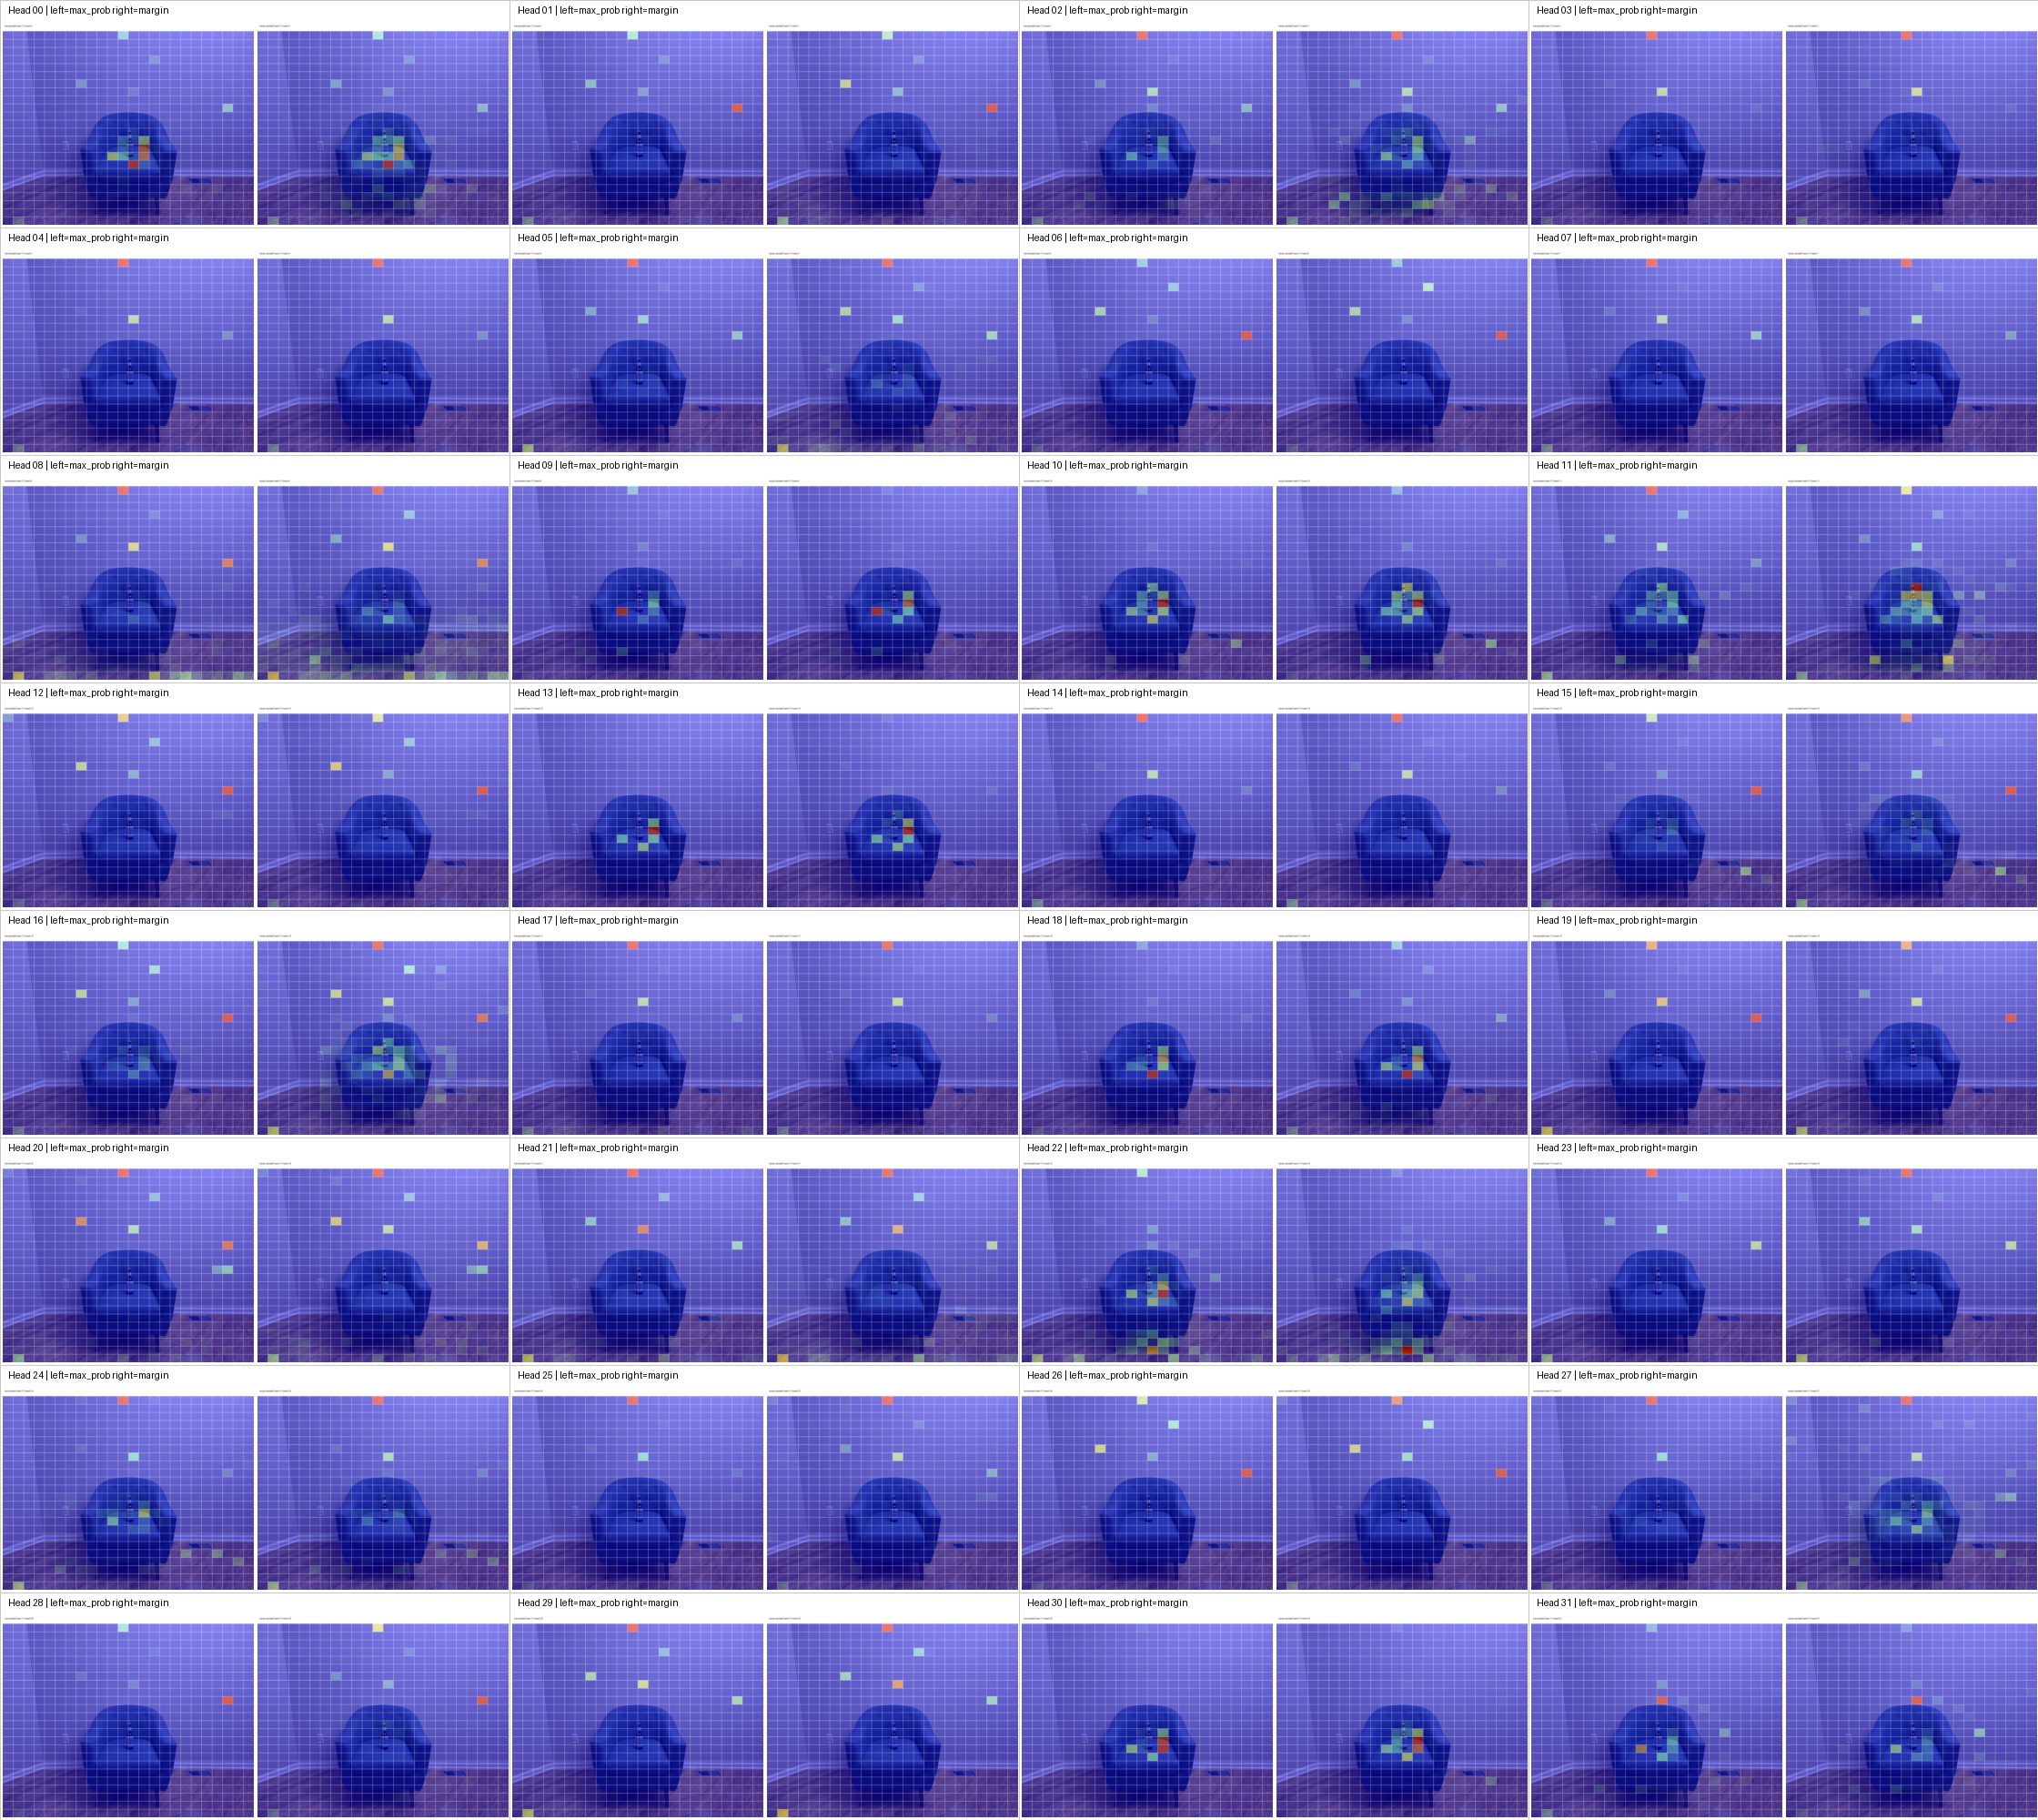
\includegraphics[width=\textwidth]{figures/head32_compare_max_vs_margin_sample0.png}
  \caption{32-head qualitative comparison on a representative controlled sample (layer 17).}
  \label{fig:head32}
\end{figure}

At dataset level, overlap ranking is dominated by heads
\{2, 18, 0, 30, 9, 11, 13, 10\},
as shown in Figure~\ref{fig:singlebox_overlap}.

\begin{figure}[H]
  \centering
  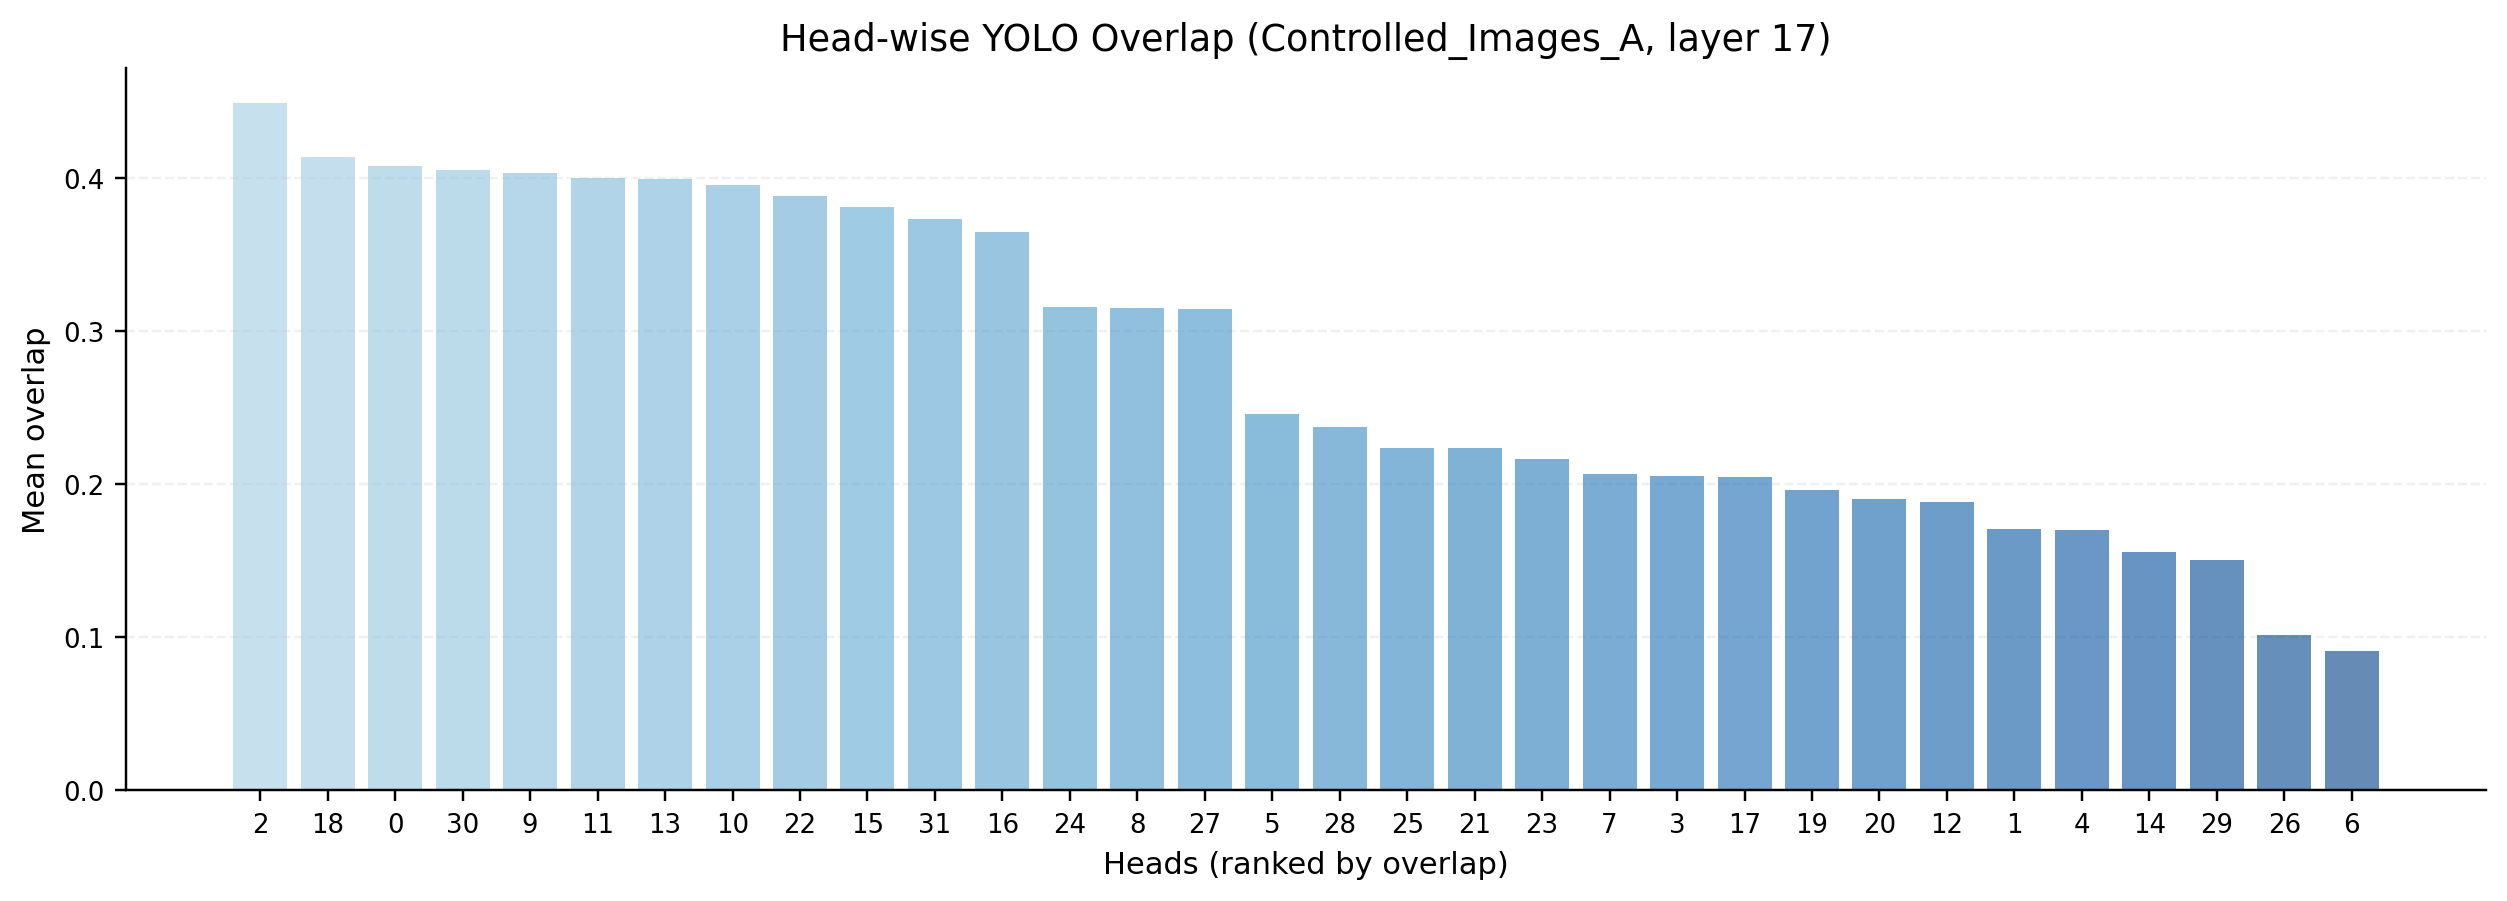
\includegraphics[width=\linewidth]{figures/control_a_head_overlap_bar_pretty.png}
  \caption{Per-head overlap on \texttt{Controlled\_Images\_A} under the single-box protocol (heads ranked by overlap; top-8 highlighted).}
  \label{fig:singlebox_overlap}
\end{figure}

\subsection{AUROC-based functional ranking}
Overlap alone does not tell us whether a head helps the final decision. We therefore evaluate each head by AUROC, using per-sample overlap scores as the predictor and answer correctness ($0/1$) as the label. Concretely, for each head $h$, we collect $\{\mathrm{Overlap}_h(x), y(x)\}_{x\in\mathcal{D}}$, where $y(x)=1$ indicates a correct answer, and compute
\begin{equation}
\mathrm{AUROC}_h = \mathrm{AUC}\big(\mathrm{Overlap}_h(x)\rightarrow y(x)\big).
\end{equation}
Top AUROC heads are
\{14, 29, 26, 6, 7, 4, 20, 17\}
(contrast visible in Figures~\ref{fig:inverse_relation} and \ref{fig:inverse_line}), which is almost disjoint from the top-overlap group.

This contrast is not anecdotal: overlap and AUROC are strongly negatively correlated across heads (Pearson $r\approx-0.915$), shown in Figures~\ref{fig:inverse_relation} and \ref{fig:inverse_line}. Figure~\ref{fig:inverse_line} sorts heads from low to high overlap and plots overlap/AUROC as two curves under the same head order, making the inverse tendency visually explicit. This is a surprising result and suggests that heads with already strong spatial concentration are not necessarily the ones most tied to final correctness.

\begin{figure}[H]
  \centering
  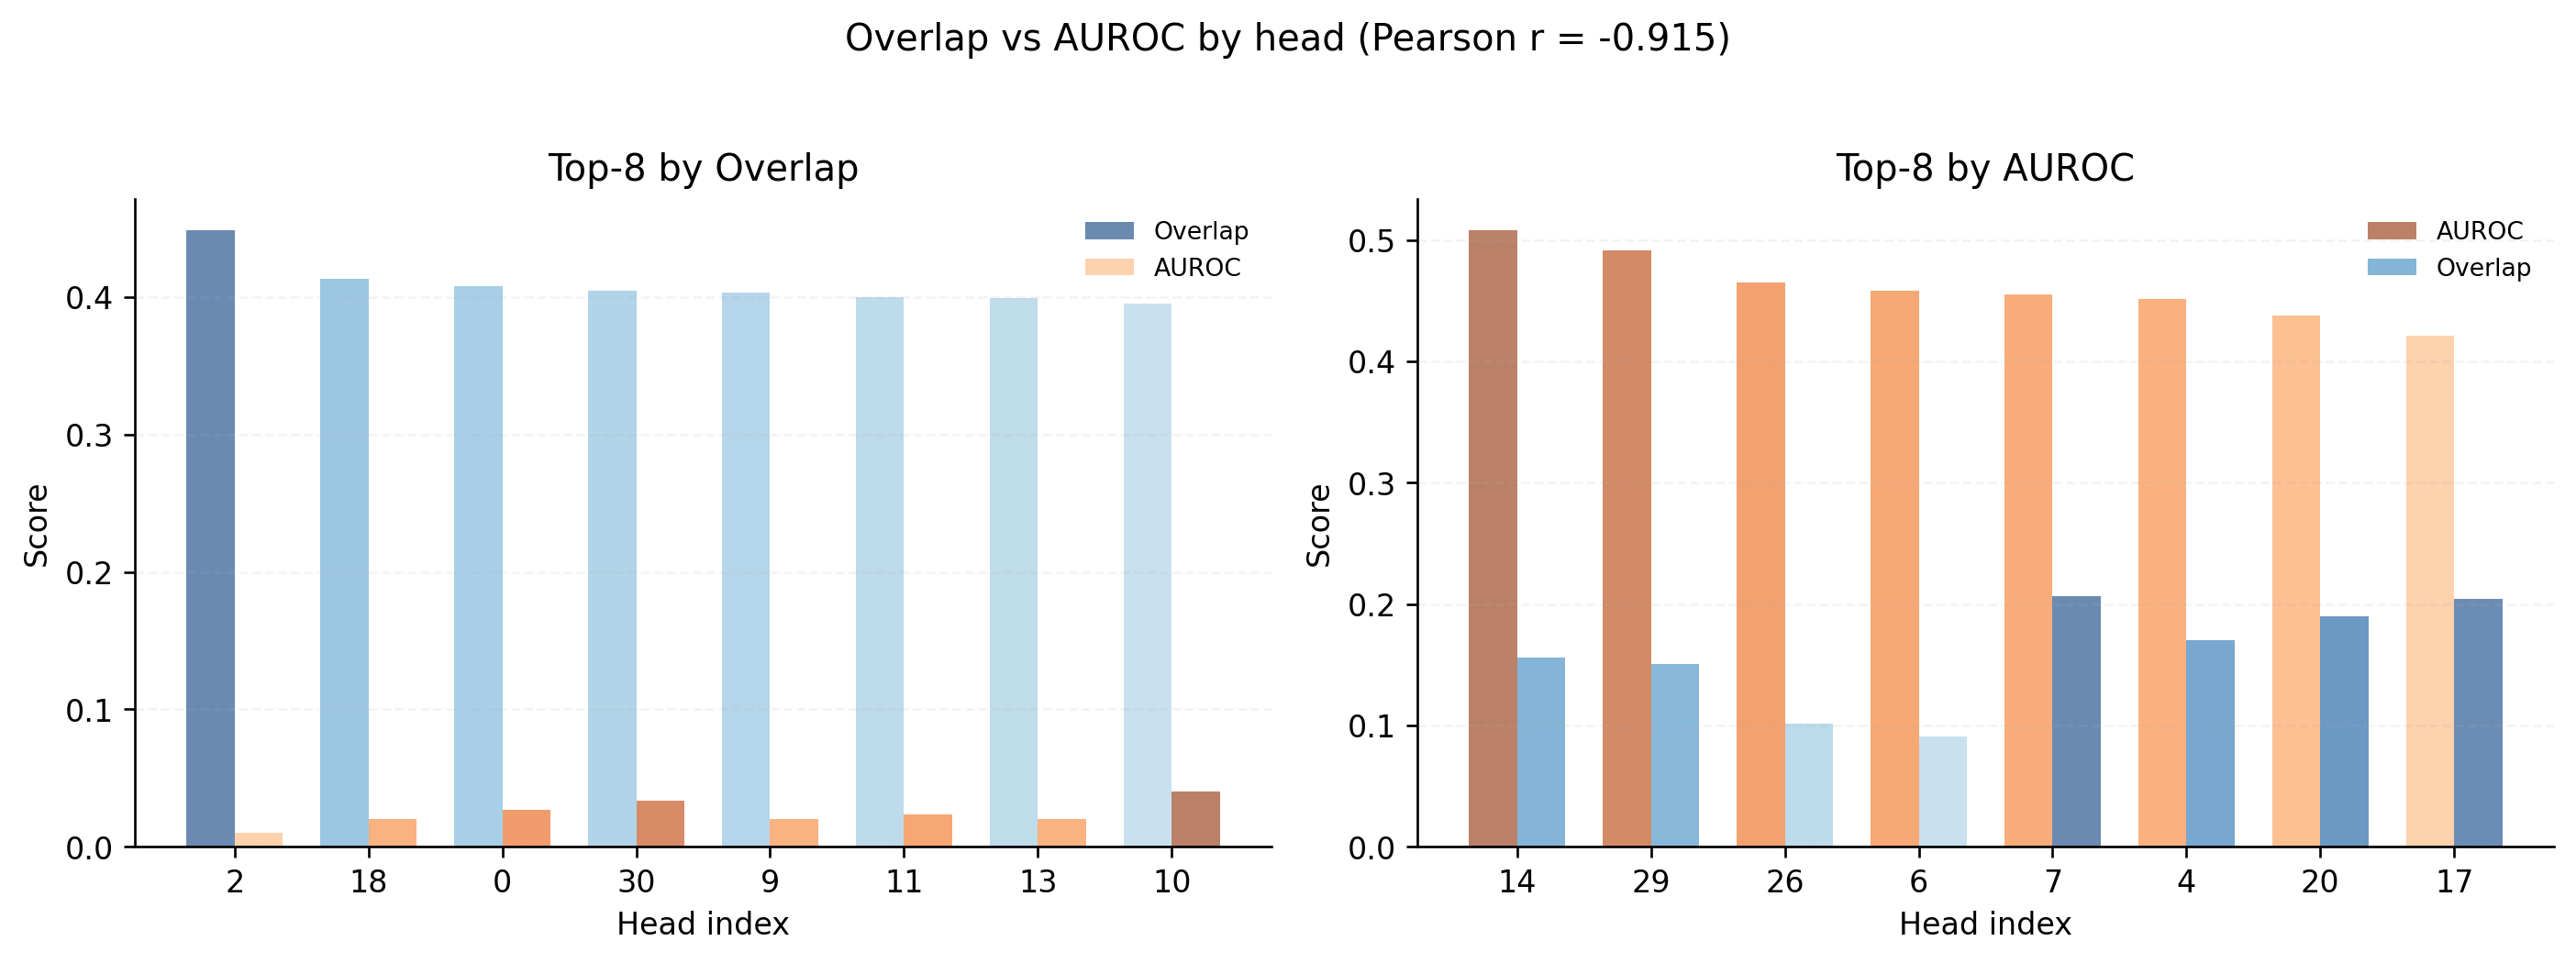
\includegraphics[width=\linewidth]{figures/head_overlap_auroc_inverse_bar.png}
  \caption{Inverse relation between overlap and AUROC across heads (top-8 overlap vs top-8 AUROC groups).}
  \label{fig:inverse_relation}
\end{figure}

\begin{figure}[H]
  \centering
  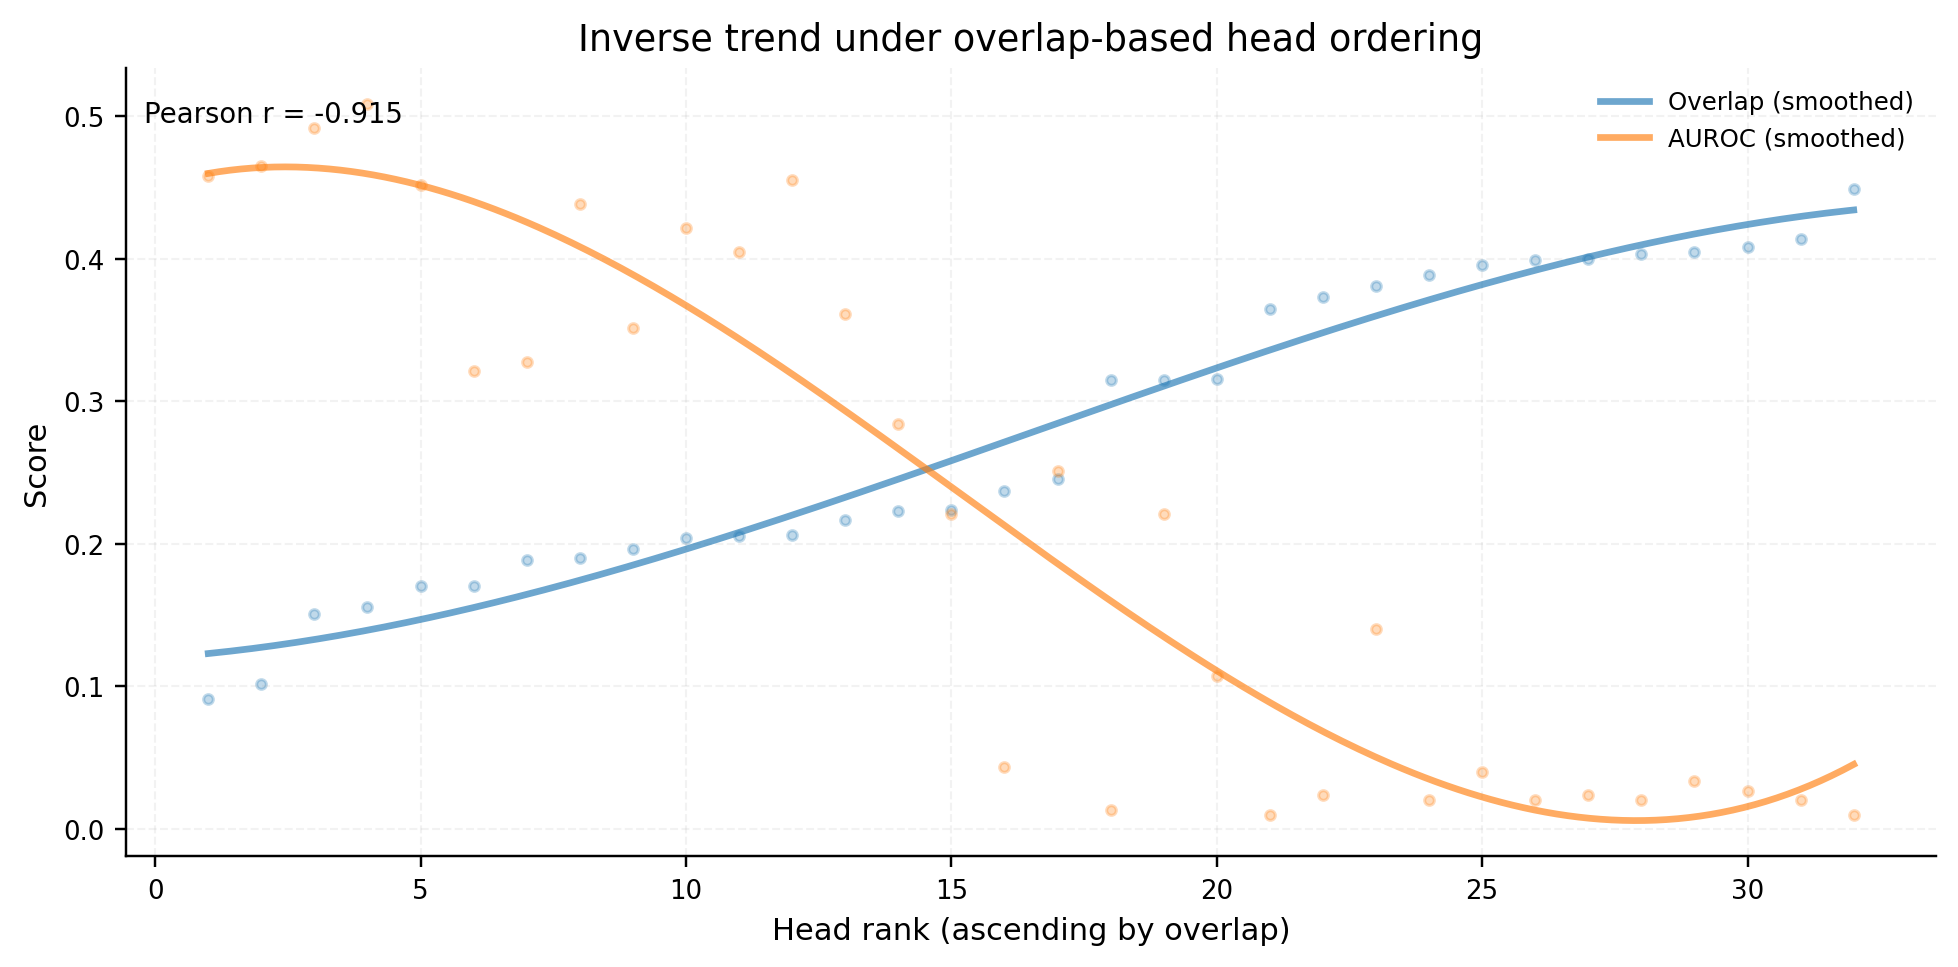
\includegraphics[width=\linewidth]{figures/head_overlap_sorted_dual_line.png}
  \caption{Two-line view of inverse relation: heads are sorted by overlap (small to large), while overlap (blue) and AUROC (orange) are plotted on the same head order.}
  \label{fig:inverse_line}
\end{figure}

\textbf{A correctly solved sample is often supported not by heads with already strong spatial attention, but by heads with weaker current spatial focus yet higher functional potential.}

\section{Our Method: Function-Aware Spatial Attention Reallocation}
\textbf{Experiment settings.}
Unless otherwise specified, this section follows the same evaluation setup as Section 3: \texttt{llava1.5}, the AdaptVis protocol, and matched 100-sample splits for cross-method comparison. We evaluate on four benchmarks with increasing relational difficulty: \texttt{COCO\_QA\_one\_obj} and \texttt{VG\_QA\_one\_obj} (single-object relation queries), and \texttt{COCO\_QA\_two\_obj} and \texttt{VG\_QA\_two\_obj} (two-object relation queries). This split allows us to check whether a method is robust only on simpler one-object questions or still effective when relational interference increases.

\textbf{Naive idea.}
Our first idea was straightforward: directly boost attention inside the YOLO box. If a region detector marks the target object, increasing weight in that region seems likely to help spatial reasoning. In practice, this direct strategy is unstable and often hurts semantic consistency; therefore, we do not include its detailed quantitative results in the main text.

\subsection{Margin-Guided Continuous Reallocation}
To address the failure mode above, we replace hard region forcing with a confidence-aware and smooth reallocation mechanism.

\textbf{(i) Margin-guided continuous control.}
At decoding step $t$, let $p_{(1),t}$ and $p_{(2),t}$ be top-1 and top-2 token probabilities. We define confidence margin
\begin{equation}
  m_t = p_{(1),t} - p_{(2),t}.
\end{equation}
Intervention strength is then set continuously by
\begin{equation}
  \alpha_t = \alpha_{\min} + (\alpha_{\max} - \alpha_{\min})\cdot \sigma\!\left(\beta(m_t-\tau)\right),
\end{equation}
where $\beta$ controls slope and $\tau$ controls the transition point.

\textbf{(ii) Attention reweighting without hard clipping.}
Given image-side attention $A_t$, we apply
\begin{equation}
  \tilde{A}_t = \mathrm{Normalize}\!\left(A_t^{\alpha_t}\right),
\end{equation}
which is the core execution step of our method: the confidence-controlled exponent $\alpha_t$ is converted into a smooth redistribution of attention mass over image patches. In practice, $\alpha_t>1$ sharpens attention to concentrate evidence, while smaller values keep attention diffuse, avoiding abrupt region-level clipping.

\subsection{Experimental Results}
Table~\ref{tab:four_dataset_main} reports the 100-sample comparison on four benchmarks. ``LLaVA-1.5'' denotes the no-intervention model output, ``AdaptVis'' denotes the original max-prob/hard setting, and ``Ours'' denotes the best margin+continuous setting under the same evaluation protocol.

\begin{table}[H]
  \centering
  \caption{Accuracy comparison on four datasets (100-sample view).}
  \label{tab:four_dataset_main}
  \resizebox{\textwidth}{!}{%
  \begin{tabular}{lcccc}
    \toprule
    Method & COCO\_QA\_one\_obj & COCO\_QA\_two\_obj & VG\_QA\_one\_obj & VG\_QA\_two\_obj \\
    \midrule
    LLaVA-1.5 (no intervention) & -- & -- & -- & -- \\
    AdaptVis & 0.54 & 0.52 & 0.38 & 0.45 \\
    Ours (margin + continuous) & 0.54 & 0.54 & 0.38 & 0.49 \\
    \bottomrule
  \end{tabular}%
  }
\end{table}

Our method preserves performance on one-object settings and improves two-object settings (COCO\_QA\_two\_obj: +0.02; VG\_QA\_two\_obj: +0.04), which is consistent with the hypothesis that better head-level spatial responsibility allocation is most beneficial when relational complexity increases. We leave the ``LLaVA-1.5'' row as a placeholder to be filled by a no-intervention rerun under the exact same 100-sample split.

\section{Conclusion}
We provide an analysis-driven workflow: identify spatially useful heads, test targeted interventions, and evaluate trade-offs between spatial alignment and task correctness. The study contributes (i) a concrete head-analysis protocol (overlap + AUROC), (ii) a targeted attention reallocation strategy, and (iii) a set of negative and positive findings that clarify where spatial head reallocation helps or fails.

\appendix
\section{Failure Case Discussion}
An additional variant we explored is \emph{top-patch flattening}: for the top-$\rho$ fraction of patches with highest attention, enforce local smoothing toward a shared high-attention level:
\begin{equation}
  \hat{A}_t(i)=
  \begin{cases}
    (1-\lambda)\tilde{A}_t(i)+\lambda\bar{A}^{\text{top}}_t, & i\in\mathcal{P}_{\rho},\\
    \tilde{A}_t(i), & \text{otherwise}.
  \end{cases}
\end{equation}
Although this variant was intended to stabilize redistribution, it often over-flattened critical contrast and degraded answer quality (especially on two-object settings) in our current runs. We therefore treat top-patch flattening as a failure-case direction rather than part of the main method.

\section{Best Hyperparameter Selection (100-sample)}
Table~\ref{tab:best_hparams_100} summarizes the selected best hyperparameters from the 100-sample tuning summary (\texttt{baseline\_vs\_best\_4ds\_100.md}). We report the final configuration used for each dataset under the margin+continuous framework.

\begin{table}[H]
  \centering
  \caption{Best hyperparameters selected from 100-sample tuning.}
  \label{tab:best_hparams_100}
  \resizebox{\textwidth}{!}{%
  \begin{tabular}{lcccccc}
    \toprule
    Dataset & Option & $w_1$/$w_2$ & Threshold & Criterion & Adapt weighting & Token/Image settings \\
    \midrule
    COCO\_QA\_one\_obj & four & 0.5 / 1.2 & 0.08 & margin & sigmoid ($\alpha$=6, span=0.1) & window=3, agg=mean, image\_scale=1.0 \\
    COCO\_QA\_two\_obj & four & 0.5 / 1.2 & 0.12 & margin & sigmoid ($\alpha$=6, span=0.1) & window=3, agg=mean, image\_scale=1.3 \\
    VG\_QA\_one\_obj & six & 0.5 / 2.0 & 0.32 & margin & sigmoid ($\alpha$=6, span=0.1) & window=3, agg=mean, image\_scale=1.0 \\
    VG\_QA\_two\_obj & six & 0.5 / 2.0 & 0.24 & margin & sigmoid ($\alpha$=6, span=0.1) & window=3, agg=mean, image\_scale=1.0 \\
    \bottomrule
  \end{tabular}%
  }
\end{table}

\section{Appendix: Naive-Idea Evaluation (TODO)}
We plan to add a dedicated quantitative comparison for the naive YOLO in-box boosting idea in a future revision. The appendix table will report four-dataset results under the same 100-sample split as the main method, including accuracy deltas versus AdaptVis and representative failure examples.

\bibliographystyle{plainnat}
\bibliography{references}
\end{document}
